% Begin the document and set up the style of the document
\documentclass[a4paper]{article}

% Install the required packages for the document 
\usepackage{envmath}
\usepackage{esvect}
\usepackage{graphicx}
\usepackage{gensymb}
\usepackage{tikz}
\usepackage[mathcal]{euscript}
\usepackage{geometry}
\usepackage{enumitem}
\usepackage{mathtools}
\usepackage{graphicx}
\usepackage{amsmath}
\usepackage{amscd}
\usepackage{amssymb}
\usepackage{amsfonts}
\usepackage{harpoon}
\usepackage{pgf}
\usepackage{tikz}
\usepackage{mathrsfs}
\usepackage{asyalign}
\usepackage{physics}
\usepackage{enumitem}
\usepackage{xhfill}
\usepackage{accents}
\usepackage{cite}
\usepackage{url}
\usepackage[tableposition=top]{caption}
\usepackage{ifthen}
\usepackage[utf8]{inputenc}
\usepackage{tikz-3dplot}
\usetikzlibrary{patterns}
\usetikzlibrary{arrows}

% Page and style settings
\parskip=8pt
\parindent=0pt
% Right margin
\textwidth=6.25in
% Left margin
\oddsidemargin=0pt
\evensidemargin=0pt
% Bottom margin
\textheight=10in
% Top margin
\topmargin=-0.75in
\baselineskip=11pt
% end of page and other style settings

\renewcommand{\familydefault}{\sfdefault}


% Begin the text of the document
\begin{document}

% Begin the Title Page
\begin{titlepage}

\newcommand{\HRule}{\rule{\linewidth}{0.5mm}} % Defines a new command for the horizontal lines, change thickness here

\center % Center everything on the page
 
\textsc{\LARGE University of Sydney}\\[1.5cm] % Name of your university/college
\textsc{\Large MATH 1903}\\[0.5cm] % Major heading such as course name
\textsc{\large Integral Calculus and Modelling (Advanced)}\\[0.5cm] % Minor heading such as course title

\HRule \\[0.4cm]
{ \huge \bfseries Assignment 2}\\[0.4cm] % Title of your document
\HRule \\[1.5cm]

\begin{minipage}{0.4\textwidth}
\begin{flushleft} \large
\emph{Author:}
Keegan Gyoery % Your name
\\
\emph{SID:}
470413467
\end{flushleft}
\end{minipage}
~
\begin{minipage}{0.4\textwidth}
\begin{flushright} \large
\emph{Lecturer:} 
Daniel Daners % Tutor's Name
\\
\emph{Seminar:}
Carslaw Tutorial Room 361
Tuesday 1pm
\end{flushright}
\end{minipage}\\[4cm]

{\large \today}\\[3cm] % Date, change the \today to a set date if you want to be precise

\vfill % Fill the rest of the page with whitespace

\end{titlepage}

\pagenumbering{arabic}

\begin{enumerate}[label=\textbf{\arabic*.}]
	\item Consider a differentiable function $\displaystyle{f\: : \: I \rightarrow \mathbb{R}}$ on the open interval $\displaystyle{I}$. Fix a point $\displaystyle{a \in I}$. The fundamental theorem of calculus asserts that
	\begin{align*}
	f(x) & = f(a) + \int^{x}_{a}f^{\prime}(t)dt\\
	\end{align*}
	We assume that all required derivatives both exist and are continuous.

	\begin{enumerate}
		\item Using integration by parts, we are required to show that 
		\begin{align*}
		f(x) & = f(a) + f^{\prime}(a)(x-a) + \int^{x}_{a}(x-t)f^{\prime \prime}(t)dt\\
		\end{align*}
		In order to complete the required proof, we must use the identity given to us at the start of the question. Further, we label the following definitions $\displaystyle{(*)}$, which will be used to perform the integration by parts.
		\begin{align*}
		du = 1 &\hspace{5mm} u = t\\
		dv = f^{\prime \prime}(t) &\hspace{5mm} v = f^{\prime}(t)\\
		\end{align*}
		Finally, we label the following result $\displaystyle{(**)}$, which will be used to complete the proof.
		\begin{align*}
		\int^{x}_{a}xf^{\prime \prime}(t)dt & = xf^{\prime}(x) - xf^{\prime}(a)\\
		\therefore xf^{\prime}(x) & = \int^{x}_{a}xf^{\prime \prime}(t)dt + xf^{\prime}(a)\\
		\end{align*}
		The proof is then as follows.
		\begin{align*}
		f(x) & = f(a) + \int^{x}_{a}f^{\prime}(t)dt\\
		& = f(a) + \int^{x}_{a}1\cdot f^{\prime}(t)dt \hspace{5mm} \text{using $(*)$}\\
		& = f(a) + tf^{\prime}(t)\:\Big|^{x}_{a} - \int^{x}_{a}tf^{\prime \prime}(t)dt\\
		& = f(a) + xf^{\prime}(x) - af^{\prime}(a) - \int^{x}_{a}tf^{\prime \prime}(t)dt\\
		& = f(a) + xf^{\prime}(a) + \int^{x}_{a}xf^{\prime \prime}(t)dt - af^{\prime}(a) - \int^{x}_{a}tf^{\prime \prime}(t)dt \hspace{5mm} \text{using $(**)$}\\
		& = f(a) + xf^{\prime}(a) - af^{\prime}(a) + \int^{x}_{a}xf^{\prime \prime}(t)dt - \int^{x}_{a}tf^{\prime \prime}(t)dt\\
		& = f(a) + f^{\prime}(a)(x-a) + \int^{x}_{a}(x-t)f^{\prime \prime}(t)dt\\
		\end{align*}
		Thus the required result is proven.

		\pagebreak

		\item We are now required to show by induction for $\displaystyle{n \in \mathbb{N}}$, that
		\begin{align*}
		f(x) & = f(a) + f^{\prime}(a)(x-a) + \frac{f^{\prime \prime}(a)}{2}(x-a)^2 + \dots + \frac{f^{(n)}(a)}{n!}(x-a)^n + \int^{x}_{a}\frac{f^{(n+1)}(t)}{n!}(x-t)^ndt \\
		\end{align*}
		In order to complete the induction, we first start with $\displaystyle{n = 1}$. This result has been proved in part $\displaystyle{(a)}$. We now shall assume that the result holds for $\displaystyle{n=k}$.
		\begin{align*}
		f(x) & = f(a) + f^{\prime}(a)(x-a) + \frac{f^{\prime \prime}(a)}{2}(x-a)^2 + \dots + \frac{f^{(k)}(a)}{k!}(x-a)^k + \int^{x}_{a}\frac{f^{(k+1)}(t)}{k!}(x-t)^kdt \dots \dots (1)\\
		\end{align*}
		Now we are required to prove the result for $\displaystyle{n=k+1}$.
		\begin{align*}
		f(x) & = f(a) + f^{\prime}(a)(x-a) + \frac{f^{\prime \prime}(a)}{2}(x-a)^2 + \dots + \frac{f^{(k)}(a)}{k!}(x-a)^k\\ 
		& \phantom{=} + \frac{f^{(k+1)}(a)}{(k+1)!}(x-a)^{k+1} + \int^{x}_{a}\frac{f^{(k+2)}(t)}{(k+1)!}(x-t)^{k+1}dt\\
		\therefore LHS & = f(x)\\
		& = f(a) + f^{\prime}(a)(x-a) + \frac{f^{\prime \prime}(a)}{2}(x-a)^2 + \dots + \frac{f^{(k)}(a)}{k!}(x-a)^k\\ 
		& \phantom{=} + \int^{x}_{a}\frac{f^{(k+1)}(t)}{k!}(x-t)^kdt \hspace{5mm}\text{by assumption $(1)$}\\
		& = f(a) + f^{\prime}(a)(x-a) + \frac{f^{\prime \prime}(a)}{2}(x-a)^2 + \dots + \frac{f^{(k)}(a)}{k!}(x-a)^k\\ 
		& \phantom{=} - \frac{f^{(k+1)}(t)}{(k+1)k!}(x-t)^{k+1}\bigg|^{x}_{a} + \int^{x}_{a}\frac{f^{(k+2)}(t)}{(k+1)k!}(x-t)^{k+1}dt\\
		& = f(a) + f^{\prime}(a)(x-a) + \frac{f^{\prime \prime}(a)}{2}(x-a)^2 + \dots + \frac{f^{(k)}(a)}{k!}(x-a)^k\\ 
		& \phantom{=} + \frac{f^{(k+1)}(a)}{(k+1)!}(x-a)^{k+1} + \int^{x}_{a}\frac{f^{(k+2)}(t)}{(k+1)!}(x-t)^{k+1}dt\\
		& = RHS\\
		\therefore LHS & = RHS\\
		\end{align*}
		Thus from the assumption of $\displaystyle{n=k}$, we have shown $\displaystyle{n=k+1}$ is also true. Thus the proof by induction is complete.


	\end{enumerate}

	\pagebreak

	\item Consider the differential equation
	\begin{align*}
	y^{\prime} & = \frac{xy(y-4)}{4}\\
	\end{align*}

	\begin{enumerate}
		\item The figure that follows is the direction field of the above differential equation between $\displaystyle{-4 \leq x \leq 4}$ and $\displaystyle{-2 \leq y \leq 6}$.

		\bigbreak


		The equilibrium solutions occur at $\displaystyle{y=0}$ and $\displaystyle{y=4}$, and thus it is easiest to examine the direction field in relation to these solutions. Thus, firstly examining the section where $\displaystyle{y > 4}$ and $\displaystyle{x > 0}$, for $\displaystyle{y}$ values slightly larger than 4, the derivative is only slightly positive, thus the direction field has small positive gradients. As the value of $\displaystyle{y}$ increases, above 4, the gradient increases and thus the directional field lines get steeper as $\displaystyle{y}$ increases.

		\bigbreak

		If we now consider the region $\displaystyle{y> 4}$ and $\displaystyle{x<0}$, we get the same results as above, except now the fact that $\displaystyle{x<0}$ means the derivative is negative, and thus the slope lines have the same magnitude for the differing y values as the region for $\displaystyle{x>0}$, but the opposite direction, that is the negative direction.

		\bigbreak

		Next, the region $\displaystyle{0<y<4}$ and $\displaystyle{x<0}$ means that the derivative is positive for all values of $\displaystyle{y}$ and $\displaystyle{x}$ that lie in these ranges. As $\displaystyle{y}$ is slightly greater than 0, the derivative has a small positive value, and thus the direction field's slope lines are shallow positive lines. As the value of $\displaystyle{y}$ increases towards 4, the magnitude of the derivative increases, and thus the slope lines increase to reflect the increasing gradient. As the value of $\displaystyle{y}$ approaches 4, the magnitude of the derivative decreases, and becomes less positive, reflected in the decreasing gradient of the slope lines.

		\bigbreak

		As before, the region with $\displaystyle{0<y<4}$ and $\displaystyle{x>0}$ behaves the same as the corresponding side of the $\displaystyle{y}$ axis, except with the derivative being negative, and hence the slope lines are negative in gradient.

		\bigbreak

		Now, for the region $\displaystyle{y < 0}$ and $\displaystyle{x>0}$, the derivative is positive for the region. When $\displaystyle{y}$ is close to 0, the gradient is slightly positive, hence the shallow slope lines. As $\displaystyle{y}$ decreases in value and becomes more negative, the magnitude of the gradient increases, reflected in the increasing positive slope of the slope lines. 

		\bigbreak

		Again, for the region $\displaystyle{y < 0}$ and $\displaystyle{x<0}$, it behaves in the same way as its corresponding region across the $\displaystyle{y}$ axis, except that the derivative is negative for this region, and thus the slope lines have a negative gradient.

		\bigbreak

		As it can be seen, as the value of $\displaystyle{x}$ approaches zero from either side, the magnitude of the derivative decreases towards zero as at $\displaystyle{x=0}$, the derivative is also 0.

		\pagebreak

		\begin{figure}[h!]
		\begin{center}
		\caption{Direction Field}
		\includegraphics[width=\linewidth]{DirectionField1}
		\end{center}
		\end{figure}

		\bigbreak

		\item We are now required to find the general solution to the differential equation given in the question.
		\begin{align*}
		\frac{dy}{dx} & =  \frac{xy(y-4)}{4}\\
		\therefore \frac{dy}{y(y-4)} & =  \frac{xdx}{4}\\
		\therefore \int \frac{dy}{y(y-4)} & = \int \frac{xdx}{4}\\
		\therefore \int \frac{dy}{y(y-4)} & = \frac {1}{4}\int xdx\\
		\end{align*}
		In order to solve the above equation, and perform the integration, we must do so by using partial fractions for the integral on the LHS of the equation. The partial fractions are as follows.
		\begin{align*}
		\frac{1}{y(y-4)} & = \frac{A}{y} + \frac{B}{y-4}\\
		\therefore 1 & = A(y-4) + By\\
		\therefore 1 & = Ay - 4A + By\\
		\therefore A + B & = 0 \dots \dots (1) \hspace{5mm} \text{equating coefficients}\\
		\therefore -4A & = 1 \dots \dots (2) \hspace{5mm} \text{equating coefficients}\\
		\therefore A & = -B \dots \dots (3) \hspace{5mm} \text{from (1)}\\
		\therefore A & = \frac{-1}{4} \hspace{5mm} \text{from (2)}\\
		\therefore B & = \frac{1}{4} \hspace{5mm} \text{from (3)}\\
		\therefore \frac{1}{y(y-4)} & = \frac{1}{4}\left[-\frac{1}{y} + \frac{1}{y-4}\right]\\
		\end{align*}
		Now we can continue with the integration from above.
		\begin{align*}
		\therefore \int \frac{dy}{y(y-4)} & = \frac {1}{4}\int xdx\\
		\therefore \frac{1}{4} \int \left[-\frac{1}{y} + \frac{1}{y-4}\right]dy & = \frac {1}{4}\int xdx\\
		\therefore \int \left[\frac{1}{y-4}-\frac{1}{y}\right]dy & = \int xdx\\
		\ln{(y-4)} - \ln{y} & = \frac{x^2}{2} + C\\
		\therefore \ln{\left(\frac{y-4}{y} \right)} & = \frac{x^2}{2} + C\\
		\therefore \frac{y-4}{y} & = \exp(\frac{x^2}{2} + C)\\
		& = \exp(C)\exp(\frac{x^2}{2})\\
		& = D\exp(\frac{x^2}{2})\\
		\therefore y - 4 & = yD\exp(\frac{x^2}{2})\\
		\therefore 4 & = y - yD\exp(\frac{x^2}{2})\\
		\therefore 4 & = y\left[1 - D\exp(\frac{x^2}{2})\right]\\
		\therefore y & = \frac{4}{1 - D\exp(\frac{x^2}{2})}\\
		\end{align*}
		Thus this final result is the general solution for the differential equation.

		\bigbreak

		\item We are now required to find the particular solution to the differential eqaution with initial value $\displaystyle{y(0) = 2}$. The derivation is then as follows.
		\begin{align*}
		y & = \frac{4}{1 - D\exp(\frac{x^2}{2})}\\
		2 & = \frac{4}{1 - D\exp(\frac{0^2}{2})}\\
		& = \frac{4}{1 - D}\\
		\therefore 4 & = 2(1-D)\\
		\therefore 4 & = 2 - 2D\\
		\therefore D & = -1\\
		\therefore y & = \frac{4}{1 + \exp(\frac{x^2}{2})}\\
		\end{align*}
		This is the particular solution to the differential equation, with intial condition $\displaystyle{y(0) = 2}$.

		\pagebreak

		\item The equilibrium solutions occur when $\displaystyle{\frac{dy}{dx}=0}$. Thus the derivation of the equilibrium points are as follows.
		\begin{align*}
		\frac{dy}{dx} & = \frac{xy(y-4)}{4}\\
		\therefore \frac{xy(y-4)}{4} & = 0\\
		\therefore xy(y-4) & = 0\\
		\end{align*}
		Thus the equilibrium points occur at $\displaystyle{y=0}$ and $\displaystyle{y=4}$. The equilibrium that occurs at $\displaystyle{y=4}$ is a divergent equilibrium, and thus is not stable. This means that for any initial value of $\displaystyle{y}$ that is in the neighbourhood of $\displaystyle{y=4}$, the solution will move away from the equilibrium solution $\displaystyle{y=4}$, as is evident by the slope lines in the direction field.

		\bigbreak

		The equilibrium point at $\displaystyle{y=0}$ is a convergent equilibrium, and thus is stable. This means that for any initial value of $\displaystyle{y}$ in the neighbourhood of $\displaystyle{y=0}$, the solution will move toward the equilibrium solution $\displaystyle{y=0}$, and tend to it as $\displaystyle{x}$ moves to either infinity.

		\bigbreak

		Whilst $\displaystyle{x=0}$ provides a solution to $\displaystyle{\frac{dy}{dx}=0}$, it is not considered an equilibrium solution, as it is not of the form $\displaystyle{y = y_0}$, for some constant $\displaystyle{y_0}$.


	\end{enumerate}

	\pagebreak

	\item A perfectly flexible and weightless cable is suspended at points $\displaystyle{A}$ and $\displaystyle{B}$. A uniform load density of $\displaystyle{\rho}$ per length is suspended from the cable, exerting a force in the vertical direction. We assume that the shape of the cable can be described by the graph of a smooth function $\displaystyle{f\: : \: (a,b) \rightarrow \mathbb{R}}$. To find an equation for the shape, we need to look at the balance of forces on the section of the cable between $\displaystyle{x}$ and $\displaystyle{x+\Delta x}$. We let $\displaystyle{T(x)}$ be the magnitude of the tension force of the cable in the direction of the tangent of the cable at $\displaystyle{(x,f(x))}$. Let $\displaystyle{\alpha = \alpha(x)}$ be the angle the tangent makes with the horizontal and note that $\displaystyle{\tan{\alpha} = f^{\prime}(x)}$.

	\begin{enumerate}
		\item We are required to firstly explain why the force acting in the horizontal direction on the cable is constant in $\displaystyle{x}$. Firstly, we must consider the system as a whole. It is clearly evident that the system is at equilibrium. As a result, there can be no net force acting on the cable at any point. This means that the horizontal components of tension at either end of the section of cable must be equal to each other. The notation $\displaystyle{\alpha_{\Delta x}}$ represents the angle between the tension at the point $\displaystyle{x + \Delta x}$, and the horizontal.

		\begin{center}
		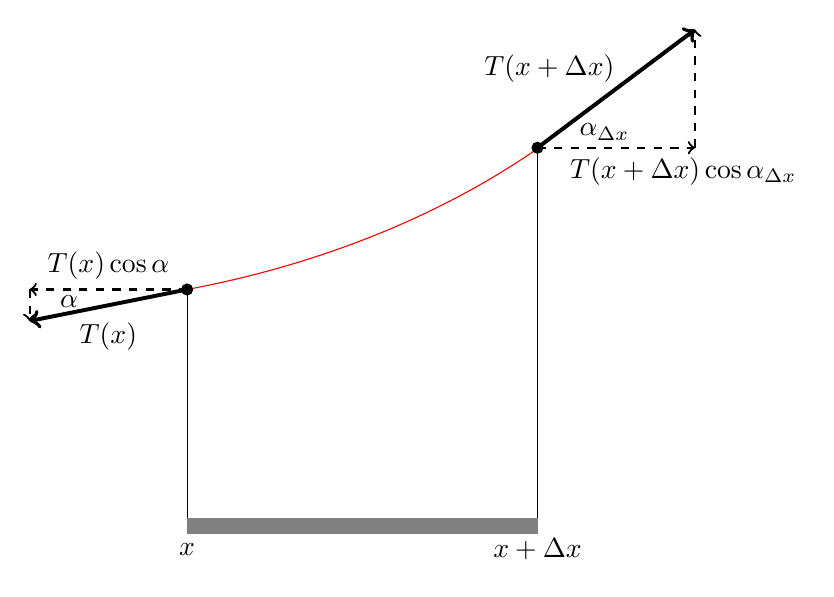
\begin{tikzpicture}

			\draw[red] (-1,0) arc (285:315:10cm and 7cm);
			\draw[fill] (-1,0) circle (0.7mm);
			\draw[fill] (3.45,1.8) circle (0.7mm);

			\draw[->][line width = 0.5mm] (-1,0) -- (-3,-0.4);
			\draw[->][line width = 0.5mm] (3.45,1.8) -- (5.45,3.3);

			\draw[->][dashed][thick] (-1,0) -- (-3,0);
			\draw[->][dashed][thick] (-3,0) -- (-3,-0.4);

			\draw[->][dashed][thick] (3.45,1.8) -- (5.45,1.8);
			\draw[->][dashed][thick] (5.45,1.8) -- (5.45,3.3);

			\draw (-1,0) -- (-1,-3);
			\draw (3.45,1.8) -- (3.45,-3);

			\node at (-1,-3.3) {$x$};
			\node at (3.45,-3.3) {$x + \Delta x$};
			\node at (-2.5,-0.15) {$\alpha$};
			\node at (-2,-0.6) {$T(x)$};
			\node at (-2,0.3) {$T(x)\cos{\alpha}$};
			\node at (4.3,2) {$\alpha_{\Delta x}$};
			\node at (3.6,2.8) {${T(x +\Delta x)}$};
			\node at (5.3,1.5) {$T(x +\Delta x)\cos{\alpha_{\Delta x}}$};

			\draw[gray][line width = 2mm] (-1,-3) -- (3.45,-3);

		\end{tikzpicture}
		\end{center}

		\bigbreak

		Using the diagram above, it is clear we have the following results.
		\begin{align*}
		\sum F_x & = 0\\
		\therefore T(x)\cos{\alpha} - T(x+\Delta x)\cos{\alpha_{\Delta x}} & = 0\\
		\therefore T(x)\cos{\alpha} & = T(x+\Delta x)\cos{\alpha_{\Delta x}}\\
		\end{align*}
		As a result of this equality, it is clear that the horizontal component of tension is independent of the choice of $\displaystyle{\Delta x}$. Thus the horizontal component of tension is a constant in $\displaystyle{x}$, that is, $\displaystyle{T(x)\cos{\alpha} = H}$, for some constant $\displaystyle{H}$.

		\bigbreak

		We are also required to deduce that $\displaystyle{T(x) = H\sqrt{1+\left[f^{\prime}(x)\right]^2}}$ for some constant $\displaystyle{H}$. Using the result from above, we get the following conclusions.
		\begin{align*}
		T(x)\cos{\alpha} & = H\\
		\therefore T(x) & = \frac{H}{\cos{\alpha}}\\
		& = H\sec{\alpha}\\
		& = H\sqrt{\sec^2{\alpha}}\\
		& = H\sqrt{1 + \tan^2{\alpha}}\\
		\therefore T(x) & = H\sqrt{1 + \big[f^{\prime}(x)\big]^2} \hspace{5mm} \text{as $\displaystyle{\tan{\alpha} = f^{\prime}(x)}$}\\
		\end{align*}
		Thus the required result is proven.

		\bigbreak

		\item We are now required to explain the forces acting on the segment of the cable between $\displaystyle{x}$ and $\displaystyle{x + \Delta x}$. The required result is $\displaystyle{H\left(f^{\prime}(x+\Delta x) - f^{\prime}(x) \right) = \rho g \Delta x}$. In order to explain the vertical forces and prove the result, the following diagram will be used.

		\bigbreak

		\begin{center}
		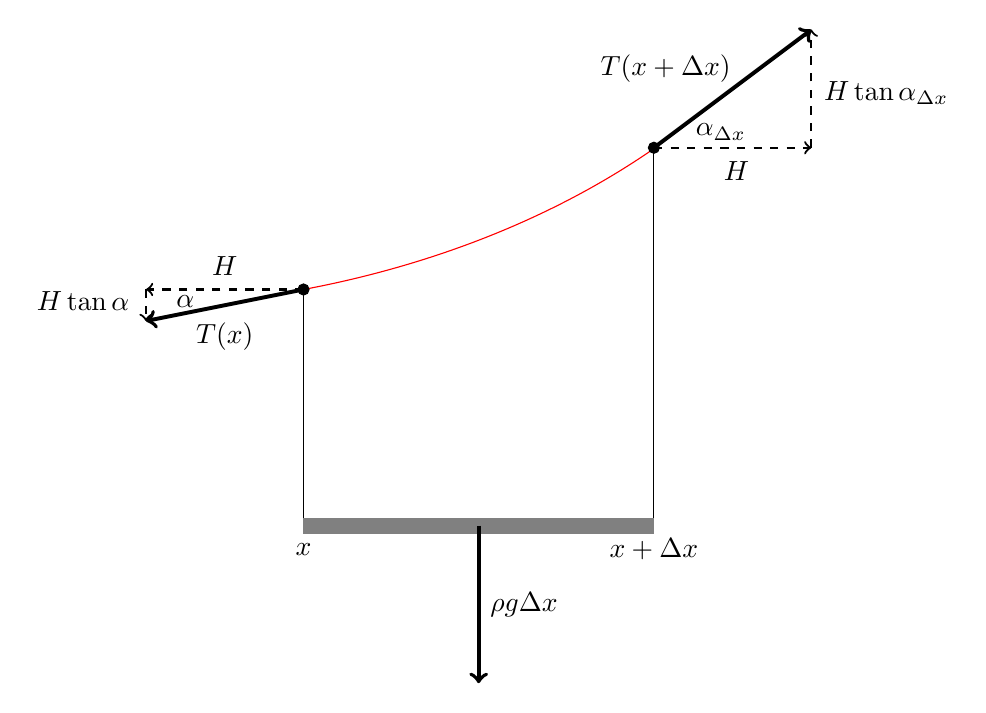
\begin{tikzpicture}

			\draw[red] (-1,0) arc (285:315:10cm and 7cm);
			\draw[fill] (-1,0) circle (0.7mm);
			\draw[fill] (3.45,1.8) circle (0.7mm);

			\draw[->][line width = 0.5mm] (-1,0) -- (-3,-0.4);
			\draw[->][line width = 0.5mm] (3.45,1.8) -- (5.45,3.3);

			\draw[->][dashed][thick] (-1,0) -- (-3,0);
			\draw[->][dashed][thick] (-3,0) -- (-3,-0.4);

			\draw[->][dashed][thick] (3.45,1.8) -- (5.45,1.8);
			\draw[->][dashed][thick] (5.45,1.8) -- (5.45,3.3);

			\draw (-1,0) -- (-1,-3);
			\draw (3.45,1.8) -- (3.45,-3);

			\node at (-1,-3.3) {$x$};
			\node at (3.45,-3.3) {$x + \Delta x$};
			\node at (-2.5,-0.15) {$\alpha$};
			\node at (-2,-0.6) {$T(x)$};
			\node at (-2,0.3) {$H$};
			\node at (-3.8,-0.15) {$H\tan{\alpha}$};
			\node at (4.3,2) {$\alpha_{\Delta x}$};
			\node at (3.6,2.8) {${T(x +\Delta x)}$};
			\node at (4.5,1.5) {$H$};
			\node at (6.4,2.5) {$H\tan{\alpha_{\Delta x}}$};

			\draw[gray][line width = 2mm] (-1,-3) -- (3.45,-3);

			\draw[->][line width = 0.5mm] (1.225,-3) -- (1.225,-5);
			\node at (1.8,-4) {$\rho g \Delta x$};

		\end{tikzpicture}
		\end{center}

		\bigbreak

		From this graph, and from part $\displaystyle{(a)}$, it is clear that the horizontal forces on the segment are equal in magnitude and opposite in direction, and thus they have no net effect on the system, which agrees with the fact that the system is in equilibrium. Furthermore, by summing the forces in the $\displaystyle{y}$ direction, we get the following results.
		\begin{align*}
		H\tan{\alpha_{\Delta x}} & = H\tan{\alpha} + \rho g \Delta x\\
		\therefore H\tan{\alpha_{\Delta x}} - H\tan{\alpha} & = \rho g \Delta x\\
		\therefore H\left(\tan{\alpha_{\Delta x}} - \tan{\alpha} \right) & = \rho g \Delta x\\
		\therefore H\left(f^{\prime}(x+\Delta x) - f^{\prime}(x) \right) & = \rho g \Delta x \hspace{5mm} \text{as $\displaystyle{\tan{\alpha} = f^{\prime}(x)}$}\\
		\end{align*}
		This is the required result for the vertical forces.

		\pagebreak

		\item We are now required to determine $\displaystyle{f(x)}$. In order to do so, we must solve the differential equation that was derived in part $\displaystyle{(b)}$. The derivation is thus as follows.
		\begin{align*}
		H\left(f^{\prime}(x+\Delta x) - f^{\prime}(x) \right) & = \rho g \Delta x\\
		\therefore \frac{f^{\prime}(x+\Delta x) - f^{\prime}(x)}{\Delta x} & = \frac{\rho g}{H}\\
		\therefore \lim_{\Delta x \to 0} \left[\frac{f^{\prime}(x+\Delta x) - f^{\prime}(x)}{\Delta x}\right] & = \lim_{\Delta x \to 0} \bigg[\frac{\rho g}{H}\bigg]\\
		\therefore f^{\prime \prime}(x) & = \frac{\rho g}{H}\\
		\therefore \frac{dy^{\prime}}{dx} & = \frac{\rho g}{H} \hspace{5mm} \text{setting $\displaystyle{y = f(x)}$}\\
		\therefore dy^{\prime} & = \frac{\rho g}{H}dx \hspace{5mm} \text{separation of variables}\\
		\therefore \int dy^{\prime} & = \int \frac{\rho g}{H}dx\\
		\therefore y^{\prime} & = \frac{\rho g}{H}x + C_1\\
		\therefore \frac{dy}{dx} & = \frac{\rho g}{H}x + C_1\\
		\therefore dy & = \bigg[\frac{\rho g}{H}x + C_1\bigg]dx \hspace{5mm} \text{separation of variables}\\
		\therefore \int dy & = \int \bigg[\frac{\rho g}{H}x + C_1\bigg]dx\\
		\therefore y & = \frac{\rho g}{2H}x^2 + C_1x + C_2\\
		\therefore f(x) & = \frac{\rho g}{2H}x^2 + C_1x + C_2\\
		\end{align*}
		Thus $\displaystyle{f(x)}$, the function that models the cable, has the shape of a parabola.

		\bigbreak

		\item We are now required to show that $\displaystyle{\int^{b}_{a}T(x)dx = HL}$, where $\displaystyle{L}$ is the length of the cable. The formula for the length of a given function, $\displaystyle{f(x)}$, between two points, $\displaystyle{a}$ and $\displaystyle{b}$, is given by $\displaystyle{\int^{b}_{a}\sqrt{1 + \big[f^{\prime}(x)\big]^2}}$. In this case, we have the result $\displaystyle{\int^{b}_{a}\sqrt{1 + \big[f^{\prime}(x)\big]^2} = L}$.

		\bigbreak

		Thus, the derivation of the result is as follows.
		\begin{align*}
		T(x) & = H\sqrt{1 + \big[f^{\prime}(x)\big]^2} \hspace{5mm} \text{from part ${(a)}$}\\
		\therefore \int^{b}_{a}T(x)dx & = \int^{b}_{a}H\sqrt{1 + \big[f^{\prime}(x)\big]^2}dx\\
		& = H\int^{b}_{a}\sqrt{1 + \big[f^{\prime}(x)\big]^2}dx\\
		& = HL\\
		\end{align*}
		
	\end{enumerate}

\end{enumerate}



\end{document}